%%
%% This is file `mcmthesis-demo.tex',
%% generated with the docstrip utility.
%%
%% The original source files were:
%%
%% mcmthesis.dtx  (with options: `demo')
%% !Mode:: "TeX:UTF-8"
%% -----------------------------------
%%
%% This is a generated file.
%%
%% Copyright (C)
%%     2010 -- 2015 by latexstudio
%%     2014 -- 2016 by Liam Huang
%%
%% This work may be distributed and/or modified under the
%% conditions of the LaTeX Project Public License, either version 1.3
%% of this license or (at your option) any later version.
%% The latest version of this license is in
%%   http://www.latex-project.org/lppl.txt
%% and version 1.3 or later is part of all distributions of LaTeX
%% version 2005/12/01 or later.
%%
%% This work has the LPPL maintenance status `maintained'.
%%
%% The Current Maintainer of this work is Liam Huang.
%%
\documentclass{mcmthesis}
\mcmsetup{CTeX = true,   % 使用 CTeX 套装时,设置为 true
        tcn = 57868, problem = A,
        sheet = true, titleinsheet = true, keywordsinsheet = true,
        titlepage = true, abstract = true}
\usepackage{palatino}
\usepackage{caption}
\usepackage{mwe}
\usepackage{amsmath}
\usepackage{lipsum}
\usepackage{times}
\usepackage{mathptmx}
\usepackage{caption}
\usepackage{subfigure}
\usepackage{framed}

\title{Managing The Zambezi River}
\author{Kai Feng, Song Lu, Yutao Zeng}
\date{\today}
\begin{document}
\begin{abstract}
The Kariba Dam is located on the Zambezi River. As one of the largest dam in Africa, its current safety state is controversial. We assume that the Kariba Dam will be removed and replaced by a multi-dam system for the sake of safety. For a complete description of this dam system, we propose two models concerning the location of new dams and the strategy for modulating the water flow through the new dam system. In order to get the optimal solution of this problem, we take the whole Zambezi River basin as research object.\\
\indent In Model A, our primary aim is to find the optimal locations of the new dams. By looking at the elevation data and making preliminary estimates, we firstly identify the general area suitable for the construction. However, the rough estimation is apparently not enough, so we narrow the candidate area by referring to other information such as geography conditions. We also established a benchmark formula by using analytic hierarchy process. This formula is a comprehensive analysis of the terrain condition, construction cost, income and safety condition of a specific location, with high reliability. Based on this formula, we tested a series of locations within the candidate areas and choose some candidate location with higher score as our solution.\\
\indent In Model B, our primary aim is to design a modulating strategy for the multi-dam system established in the Model A. Since the water level of Zambezi River changes intensely in a year, we anticipate that it is very difficult to obtain a unified scheduling scheme directly. So, we firstly established a linear model with a global optimal solution under certain constraints. Moreover, we considered the action of the river authority and take it as a parameter. After that, we bring the historical data into our model and get the value of parameters in normal year, in the dry season and rainy season.
\begin{keywords}
Kariba Dam, AHP method, Multi-dams arrangement
\end{keywords}
\end{abstract}
\maketitle
\section{Introduction}
\indent \indent The Kariba Dam is one of the biggest dam in the world, which is constructed on the Zambezi River. It supplies 1626 megawatts of electricity to parts of both Zambia and Zimbabwe. However, the Kariba Dam is in a dangerous state now. In the past 50 years, the torrents from the spillway have eroded its bedrock, carving a vast crater that has undercut the dam's foundations.$^{[1]}$ A number of options are available to solve this problem. This paper focuses on the third option -- Removing the Kariba Dam and replacing it with a series of small dams along the Zambezi River. To find the best location for new dams and do the best arrangement with the multi-dam system, we propose two mathematical models. This paper describe these two models minutely and give suggestions on where to build new small dams and how to dispatch all the dams. \\

%%%%%%%%%%%%%%%%%%%%%%%%%%%%Introduction ends here%%%%%%%%%%%%%%%%%%%%%%%%%%%%%%

\section{Model A: Search for possible locations to build dams}
\subsection{Description}
\indent \indent To build new dams, we need to find some proper locations at first. However, we cannot pick all the suitable locations manually since Zambezi River is rather long. So our underlying idea is fairly simple. Firstly, we find a serial of possible river reaches. Although only a rough estimate, it does help us to exclude many reaches which cannot meet the requirements. Then we can pick some suitable locations from the reaches left. In this step, we need to refine this problem. Generally, the choice of dam's location should be related to geology, terrain, economic, ecology, disaster and other factors. Among all the factors, the dominant factor should be terrain for it decides both the safety and the economy of the reservoir. We build a formula as a benchmark to quantify their impact to the selection and pick the locations with the highest grade as our result. The following is the detailed discussion. 
\subsection{Analysis and Assumptions}
\indent \indent To be specific, we get two principle of searching for possible reaches to build dams:
\begin{enumerate}
  \setlength{\itemsep}{0pt}
  \setlength{\parsep}{0pt}
  \setlength{\parskip}{0pt}
  \item The higher the vertical drop is, the more abundant hydropower resource is contained;
  \item In consideration of reducing ecological impact and water evaporation, the surface area of reservoirs should be small under certain requirement of volume. To build reservoir with small surface area and certain volume, the average depth of reservoir should be deep, thus, dams should be built between deep ravines.
\end{enumerate}

\indent Hydropower station convert gravity potential of water into electrical energy. The gravity potential is calculated as $E_{p} = mgh$, thus, higher vertical drop means bigger electricity-generation capacity. In order to simplify the expression, all symbol used in this model are listed in the table below.\\
\begin{table}[ht]
\centering
  \begin{tabular}{cc}
  \hline
  Symbols & Meanings \\
  \hline
  $V$ & the volume of reservoir \\
  $S$ & the water surface area of reservoir \\
  $H$ & the water depth of reservoir \\
  $\alpha$ & the angle of bank slope \\
  $g$ & the gravitational acceleration \\
  \hline
  \end{tabular}
\caption{Symbol Table of Model A}
\end{table}\\
\indent To simplify model, we assume that the vertical section of a reservoir is an approximate trapezoid, then the submerged area can be expressed as below:
\begin{equation}\int_{A}^{B}\frac{H\left(l\right)}{\sin\left[\alpha\left(l\right)\right]}dl + \int_{C}^{D}\frac{H\left(L\right)}{\sin\left[\alpha\left(L\right)\right]}dL + S_{bottom}\end{equation}
where $l, L$ are respectively the lengths of left bank and right bank; $A, B$ indicate the starting position and end position of $l$; similarly, $C, D$ indicate the starting position and end position of $L$.
The expression $\left(1\right)$ is still hard to use because of the difficult estimation of $\alpha$. In order to make our assessment feasible, we need to simplify the expression $\left(1\right)$. Noticed that:
\begin{equation}
\int_{A}^{B}\frac{H\left(l\right)}{\sin\left[\alpha\left(l\right)\right]}dl = \frac{1}{sin\left[\alpha\left(\zeta\right)\right]}\int_{A}^{B}H\left(l\right)dl
= KH_{average}l
\end{equation}
where $K$ is a coefficient of inclination. expressions $\left(2\right)$ is a application of mean value theorem for integrals, it fits in with the physics intuition. Then, the submerged area can be estimated as:
\begin{equation}
\left(K_{1}l + K_{2}L\right)H_{average} + S_{bottom}
\end{equation}
Using expression $\left(3\right)$, we can qualitatively explain why small surface area is needed. Using equation $H_{average} = \frac{V}{S}$, we get:
\[S_{submerged} \approx \left(K_{1}l + K_{2}L\right)\frac{V}{S} + S_{bottom}\]
and using the assumption of vertical section, the area of the bottom of a reservoir can be estimated as:\\
\begin{equation}
S_{bottom} = \int\left(\beta dS \right) \propto S
\end{equation}  
where $\beta$ is a coefficient of water surface area size and bottom area size, the expression $\left(4\right)$ qualitatively explain that $S_{bottom}$ is proportional to $S$, thus we get:\\
\begin{equation}
S_{submerged} \approx \left(K_{1}l + K_{2}L\right)\frac{V}{S} + CS
\end{equation}
where $C$ is a coefficient to indicate that $S_{bottom}$ is proportional to $S$.\\
\indent Since the right side of the expression $\left(5\right)$ is a hyperbolic function, it monotonically decrease when $S \geq \sqrt{\frac{\left(K_{1}l + K_{2}L\right)V}{C}}$. In the actual situation, $S \gg \sqrt{V}$, so we can qualitatively conclude that under certain requirement of volume small surface area of reservoir is more beneficial than the bigger surface area.\\
\indent According to the discussion above, we should find the reaches with big throws on the Zambezi river based on the first principle. In accordance with the second principle, the possible reaches should between deep ravines, because a reservoir in deep ravines can have deeper water depth and thus smaller surface area.\\
\subsection{Model Building}
\subsubsection{Search for candidate areas}
\indent \indent In order to find suitable dam sites along the Zambezi River, we established a simple model based on the geographical conditions, costs, safety of the whole dam system and other fatal conditions. \\
\indent The storage capacity of dams depends on the height of dams which is limited by the slope and height of the river bank. The cost of construction basically depends on the dam's height and length as well as the width of river. Thus, there are three major parameter to be taken into account in choosing candidate regions:
\begin{itemize}
\item The vertical drop of the river.
\item The slope and height of the river bank.
\item The width of river.
\end{itemize}

We download the geomorphological data of the Zambezi River Basin and generate a Digital Elevation Model (DEM). The Figure 1 is a general overview of the elevation in that region (the Zambezi River is marked in red line in the chart).\\
\begin{figure}[h]
\small
\centering
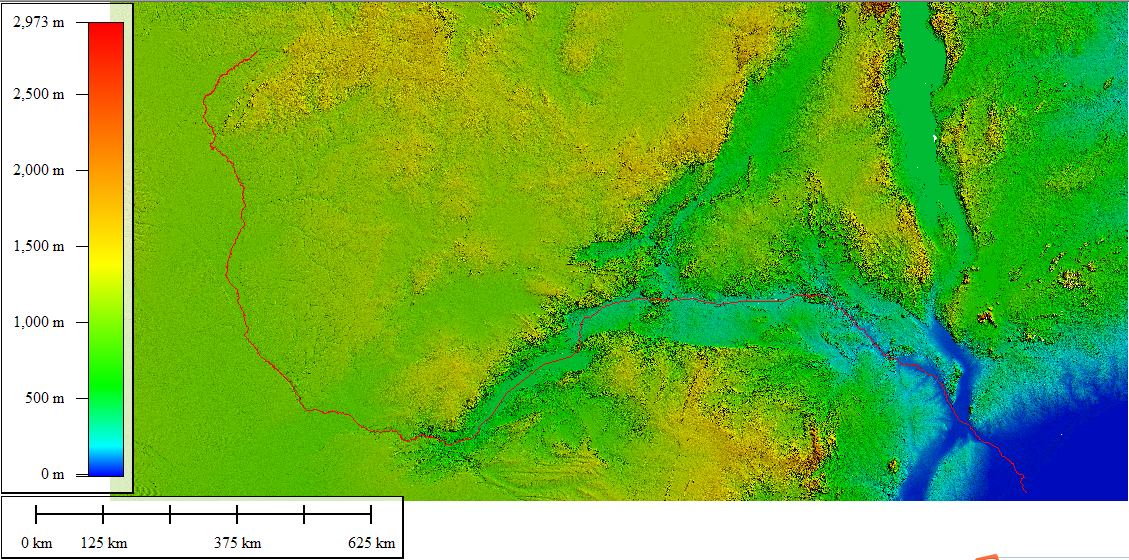
\includegraphics[width=14cm]{./figures/Sensing_Figure.png}
\caption{Overview Elevation Chart} \label{fig:Fig1}
\end{figure}
By using DEM, we obtain the elevation along the whole Zambezi River and plot the elevation figure as Figure 2. From Figure 2, We can obviously notice that the river is divided into 3 parts. There is a clear trend that the upstream is relatively plain, the water level decreases remarkably in the midstream and shoulders the most responsibility of storing water, the downstream have a rapid change of water level as well but there are few dams. Three prominent falls of the elevation are the Victoria Fall, the Kariba Dam and the Cahora Bassa Dam.

\begin{figure}[h]
\small
\centering
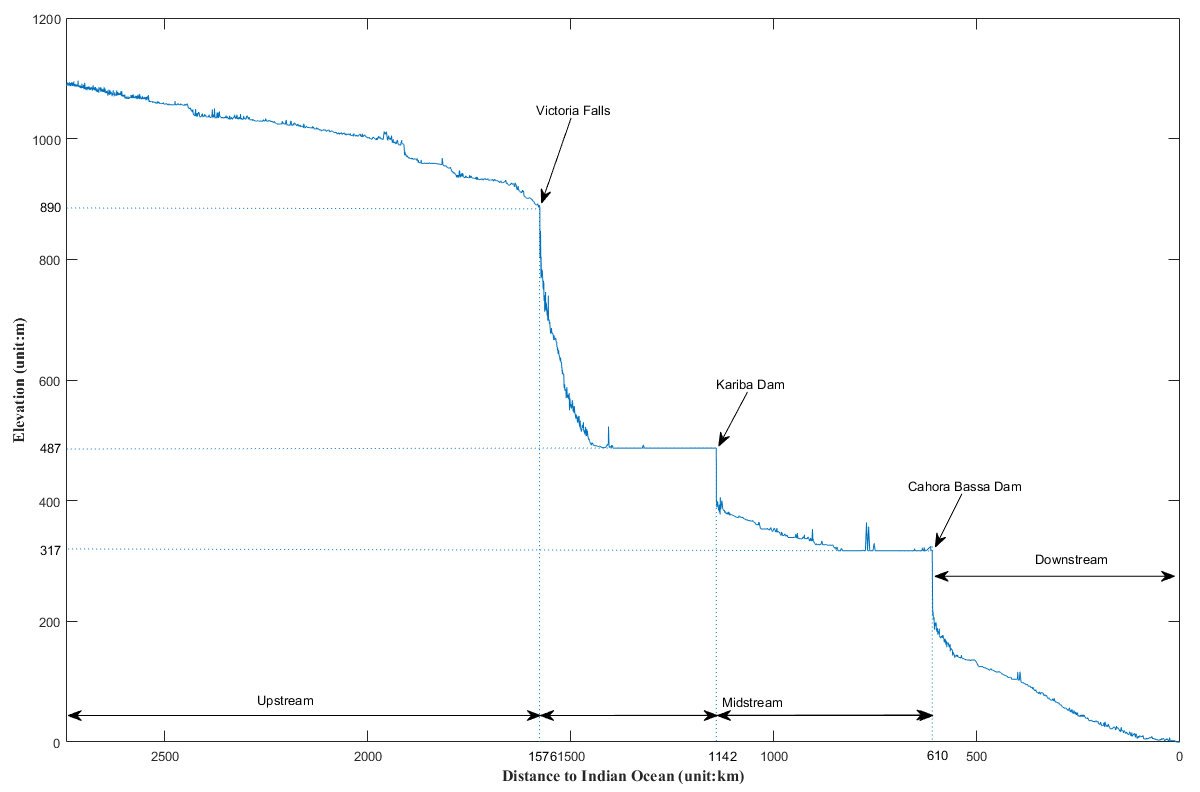
\includegraphics[width=14cm]{./figures/dis_alti_v3.png}
\caption{Elevation along the Zambezi River} \label{fig:Fig2}
\end{figure}

%%%%%%%%%%%%%%%%%attention here!%%%%%%%%%%%%%%%%%%%%%%%%%%
From the perspective of the vertical drop, we know the following areas are suitable for the establishment of dams: a few areas of upstream, reaches between Victoria Fall and Kariba Lake, reaches between Kariba Dam and Cahora Bassa Dam, some areas in the downstream. The exact areas are marked in red in Figure 3. In addition to the drop, we also need to analyze the slope and height as well as the breadth of the Zambezi River itself for they have great affect on the cost of dam construction. We plotted the contours of the Zambezi River basin based on the DEM model above. Generally, for the sake of storage capacity, safety and ecological impact, the bank of the reservoir should be steep as possible and have suitable height. The steepness of the bank means less flooded area and less impact on the surrounding environment. We also know that the dam should never be higher than the bank, so considerable height of the bank allows the reservoir to have a higher water level and proofs the robustness of the dam in extreme cases like flood. In addition, we don't expect to build our dam across a wide river. Not only because building dams in narrow valley can significantly reduce construction cost, but also since the too long dam body may have a negative impact on the safety of the dam.\\
\indent We plot the contours of Zambezi River basin by using the DEM model above. The followings are 2 samples of the whole picture whose contour interval is 5 meters. The dense the contours means the river bank is steep which is good for us to build the dam.\\

\begin{figure}[h]
\small
\centering
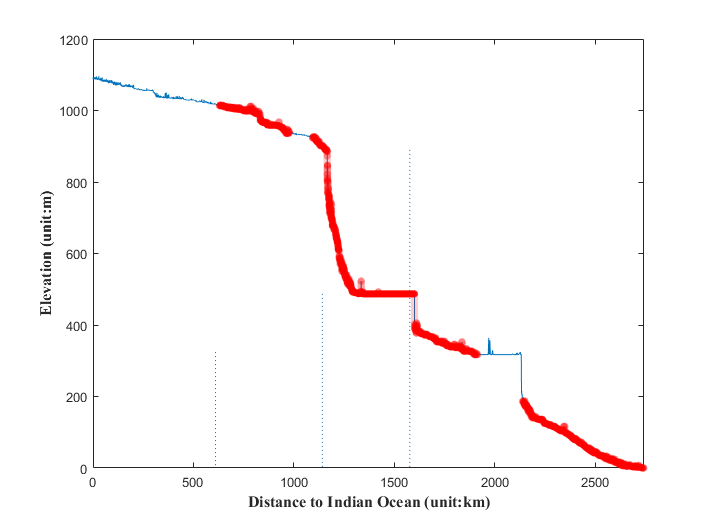
\includegraphics[width=8cm]{./figures/highlight0.png}
\caption{Candidate areas according to vertical drop} \label{fig:Fig3}
\end{figure}

\begin{figure}[htbp]
\centering %居中
\subfigure[Instance with dense contours]{ %第一张子图
\begin{minipage}{7cm}
\centering %子图居中
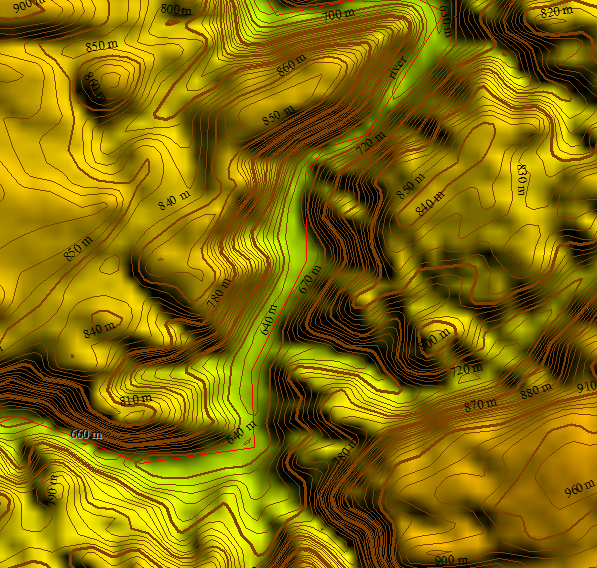
\includegraphics[scale=0.22]{figures/midstream_contour.png} %以pic.jpg的0.5倍大小输出
\end{minipage}
}
\subfigure[Instance with sparse contours]{ %第二张子图
\begin{minipage}{7cm}
\centering %子图居中
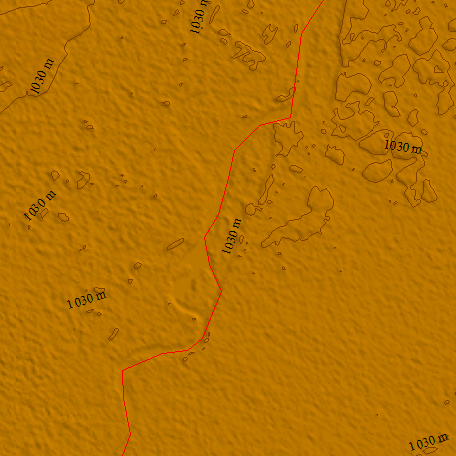
\includegraphics[scale=0.3]{figures/upstream_plain_contour.png} %以pic.jpg的0.5倍大小输出
\end{minipage}
}
\caption{Contour samples along Zambezi River} % %大图名称
\label{fig:1.3.1} %图片引用标记
\end{figure}
\indent Taking these factors into account, we further reduced the candidate areas as Figure 5.
\begin{figure}[h]
\small
\centering
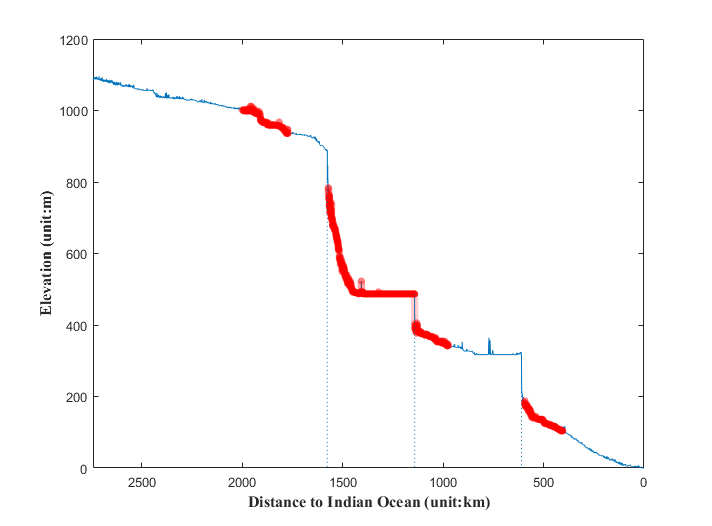
\includegraphics[width=10cm]{./figures/highlight1.png}
\caption{Candidate areas according to combined factors} \label{fig:Fig4}
\end{figure}
\indent In addition, we need to consider the geological foundation conditions on both sides of the river. The rock layer of the candidate areas are rather solid and the vegetation along the river is lush which means it is less like to happen landslide in these areas. Base on the discussion above, we don't narrow the candidate areas any more since they are suitable for the construction of dams, the next step is build a function as benchmark and pick the exact locations from these candidate areas.

\subsubsection{Building Benchmark function}
\indent \indent From the discussion above, we have obtained the candidate dam construction area. However, evaluate from the continuous area is a heavy load work with great difficulty and complexity, so we try to turn the continuous problem into discrete problem and reduce the complexity of the problem.\\

\textbf{Geography Analysis}\\
\indent The choose of the dam should based on various geographical factors, such as vertical drop, rock and soil condition, the slope and height of the bank and the width of the river etc. With so many factors to be considered, we decided to use analytic hierarchy process(AHP) to do this job.\\
\indent Firstly, we need to establish the natural coordinate along the river. We assume $l$ to be the distance from the upstream source to the the candidate point.

\begin{table}[!ht]
\centering
  \begin{tabular}{cc}
  \hline
   Intensity of Importance & meaning  \\
  \hline
  $1$ & Equal importance \\
  $3$ & Moderate importance \\
  $5$ & Strong importance \\
  $7$ & Very strong or demonstrated importance \\
  $9$ & Extreme importance \\
  $2,4,6,8$ & Intensity between two hierarchies \\
  $1,1/2,...,1/9$ & The opposite numbers\\
  \hline
  \end{tabular}
  \caption{Intensity of Importance}
\end{table}

We combined these factors into a hierarchical factor vector $\textbf{P}_1$, and get $\textbf{P}_1 = (F_{l}, \alpha_{l}, H_{l}, C_{l}, W_{l})$. Then we can get the comparison matrix $\textbf{A}_1$ which is satisfied with the following equation:
\begin{equation}
\textbf{A}_1 = (a_{i,j})_{5\times5},\qquad a_{ij} > 0, \quad a_{ij} = \frac{1}{a_{ji}}
\end{equation}
Now we need to get the importance of each factor, that is , the weight vector $\textbf{w}$. The $C_{l}$ and $W_{l}$ decides whether the construction is feasible to a great extent, so they are regarded as the most important factors. Between $W_{l}$ and $C_{l}$, $W_{l}$ has more flexibility, so we decide to choose $W_{l}$ as a more effective judge factor. In the other 3 elements, $F_{l}$ and $H_{l}$ decide they storage capacity of the dam, so they are also with a certain importance. However, $\alpha_{l}$ mainly influence the submerged area, so we think it a less significant factor. So we get the comparison matrix as below:
\[\textbf{A}_1 = 
\left[
\begin{matrix}
1 & 5 & 1 & \frac{1}{3} & \frac{1}{4} \\
\frac{1}{5}  & 1 & \frac{1}{5} & \frac{1}{7} & \frac{1}{8} \\ 
1 & 5 & 1 & \frac{1}{3} & \frac{1}{4} \\
3 & 7 & 3 & 1 & \frac{1}{2} \\
4 & 8 & 4 & 2 & 1 \\
\end{matrix}
\right]
\]
Calculating the maximum eigenvalues of matrix $A$, we get $\lambda = 5.1415$. The consistency indicators of $\textbf{A}_1$ is \[\mathit{CI} = \frac{\lambda - n}{n - 1} = 0.0354\]
where $n$ is the order of the matrix. When $n = 5$, the random consistency index \textit{RI} is $1.12$. Then the consistency ratio of matrix A is \[\mathit{CR} = \frac{\mathit{CI}}{\mathit{RI}} = 0.0316 < 0.1 \]
The error of $\textbf{A}_1$ is acceptable, and the eigenvector of $\lambda$ is $\left[0.2185, 0.063, 0.2185, 0.5190, 0.7945\right]$
Based on the calculation above, we get the weight vector $\textbf{w}_{1}$.
\begin{equation}
\textbf{w}_{1} = \lambda = \left[0.2185, 0.063, 0.2185, 0.5190, 0.7945\right]
\end{equation}
and our initial benchmark function is:
\begin{equation}
E(l) = \textbf{P}\textbf{w}_{1}^{T} = 0.2185F_l + 0.063{\alpha}_{l} + 0.2185H_l + 0.519C_l + 0.7945W_l
\end{equation}
There are something need to note when using this function:
\begin{itemize}
  \item This function can only determine \textbf{one} point each time because every selected point will change $H_l$.
  \item When establishing the function of these five factors, it is necessary to set a maximum value of this function, since the dam establishment only needs to meet the appropriate conditions. The function can be expressed as 
  \begin{eqnarray}
  F(x) =
  \begin{cases}
  f(x) & 0 < x < \theta \cr F_{max} & x \ge \theta
  \end{cases}
  \end{eqnarray}
\end{itemize}
Our location selecting algorithm are as follow:
\begin{framed}
\newcounter{alg}
\begin{list}{\arabic{alg}.}
    {\usecounter{alg}\setlength{\parsep}{0ex}\setlength{\itemsep}{0ex}}
\item[] Dam Location Selecting Algorithm
\item Create a natural coordinate system of the candidate area, and take the upstream source as the origin. The evaluation threshold is set as $T_{0}$.
\item Based on the coordinate and DEM data we get, create the function of 5 factors including $F(l),\alpha(l),H(l),C(l)$ and $W(l)$, then set the maximum value of it.
\item Bring $l$ into evaluation function $E(l)$, and select the point that satisfies the condition best as candidate point.
\item According to the obtained candidate point, divide this area into 2 segment. Repeat step 2 and step 3 to each of these segments until no new candidate points are generated.
\item Put all candidate points into candidate set.
\end{list}
\end{framed}
\textbf{Cost Analysis}\\
\indent Besides the geography conditions, we also needs to consider the cost of dam construction, including the design cost of the whole project, the overall construction cost of the project, the feasibility analysis report of the later stage of the project etc.\\
Firstly, we need to calculate the construction costs. According to the cost formula given by Hydro Review Maga, the construction cost is directly related to the size of the dam.
\begin{equation}
C_{build} = K(\frac{V_{cap}}{(H/\Delta)^{\eta}})^{\gamma}
\end{equation}
where $V_{cap}$ is the installed capacity, $H$ is the height of the water head, $\Delta$ and $\eta$ are two  coefficient to adjust the relationship between $V_{cap}$ and $H$, $\gamma$ is the cost index, $K$ is the cost coefficient. The value of $K$ often depends on the size of the dam. For example, the $K$ of the big dam is $7.7\times10^4$, while the small dam could be $5.0 \times 10^4$.
\indent We can calculate the installed capacity $V_{cap}$ based on the annual flow of the river, the detailed data can be found from the Internet. The formula to calculate $V_{total}$ is:
\begin{equation}
V_{total} = V_{flow} - V_{evap} + V_{rain} = V_{flow} - (1-{\alpha})v_{0}S({\mu}T_{aver})^{\theta} + {\beta}v_{1}S
\end{equation}
where $v_{0}$ is the evaporation of the water per day per unit area, $\alpha$ is the evaporation reflux coefficient, $\mu$ is the temperature regulation coefficient, $\beta$ is the proportion of precipitation into the reservoir, $v_{1}$ is the annual average rainfall per unit area, $S$ is the area of river, $t$ is the time.\\
\indent $S$ can be calculated by using following formula:
\begin{equation}
S \approx \left(K_{1}l + K_{2}L\right)\frac{V}{S} + CS
\end{equation}
\indent Now we get the formula to calculate the installed capacity:
\begin{equation}
V_{cap} = {\rho}gV_{total}H = {\rho}g(V_{flow} - (1 - {\alpha})v_{0}S({\mu}T_{aver})^{\theta}t + {\beta}v_{1}St)H
\end{equation}
\indent Then we consider the cost of the construction of the dam. There are some relations between the design costs and the construction cost, so we can directly get
\begin{equation}
C_{design} = {\delta}(C_{build})^{\tau}
\end{equation}
where $\delta$ is the proportional coefficient, $\tau$ is the proportional index. According to the data we get, $\tau$ generally go for 0.9 and $\delta$ generally goes for 0.34.
\indent Then we start to consider other costs when building a dam. According to the statistic given by the World Bank, the cost of feasibility report before and after the construction account for about $12\%$ of total design cost.
\begin{equation}
C_{prev} + C_{later}= (\alpha_{1} + \alpha_{2})C_{design} = 0.12C_{design}
\end{equation}
Finally, we get the total cost of the project:
\begin{equation}
C_{project} = C_{build} + C_{design} + C_{prev} + C_{later}
\end{equation}
\begin{equation}
C_{project} = K(\frac{V_{cap}}{(H/\Delta)^{\eta}})^{\gamma} + (1+\alpha_{1}+\alpha_{2}){\delta}(K(\frac{V_{cap}}{(H/\Delta)^{\eta}})^{\gamma})^{\tau}
\end{equation}\\
\textbf{Income Analysis}\\
\indent After the cost analysis, let's come to the income analysis. We can calculate the profit gained from annual power generation by using the installed capacity of the dam. 
\begin{equation}
B_{elec} = V_{cap}T_{use}p_{elec}
\end{equation}
where $T_{use}$ is the power-generation time in a year(The hydropower is stopped during the low water period.),  $p_{elec}$ is the local electricity price. Usually, $T_{use}$ is between $3700-4200$h and local electricity price is $0.384\sim0.468$Cent/KWh.
In addition, building new dams will bring some extra income such as Fishery income, tourism income, irrigation income and so on.Based on the model built by Welcomme$^{[2]}$, we can calculate the fishery income by using the equation below:
\begin{equation}
B_{fish} = {\gamma}S^{\theta}P_{fish}
\end{equation}
where $\gamma$ is the relation coefficient between watershed area and fishery output, $\theta$ is the relation index between watershed area and fishery output, $p_{fish}$ represent the local fish price on average. In this paper, $\gamma$ is set to 0.03 and $\theta$ is set to 0.97. According to the fishery data in 2016, we set $p_{fish}$ to 3.5 dollar per kilogram. There are also some benefit that cannot be quantized like the irrigation benefit and emergency response capability. \\
The final dam income formula is:
\begin{equation}
B_{total} = B_{elec} + B_{fish} + B_{other}
\end{equation}
where $B_{other}$ is a basic estimate of other benefits including the irrigation benefit and emergency response capability. Specific values can refer to other dams on the downstream of the Zambezi River.\\
\textbf{Safety Analysis}\\
\indent Since we are analyzing the impact on safety made by local terrain and geological. The evaluation function obtained above is used directly as a measure of security here.
\begin{equation}
S_{i} = E_{l,i}
\end{equation}
\textbf{Other Factors}\\
\indent At the same time, the influencing factors of people and environment should be put into out evaluation function as a measurement factor. Some of them are more prominent such as the impact of the residents living around(cost of immigration) and the animals and plants living in the submerged areas. We use the formula below to quantify the impact.
\begin{equation}
F_{other} = P_{i}({\xi}S^{\sigma})m_{0} + S_{submerge}(\beta_{1}m_{1} + \beta_{2}m_{2}) + F_{balance}
\end{equation}
where $P_{i}$ means the density of the population around the $i$th dam, ${\xi}S^{\sigma}$ is a formula used to estimate how many people will be influenced by the new dam, $S$ is the area of reservoir, $m_{0}$ is the migration costs per person, $S_{submerge}$ is the size of submerged area, $\beta_{1} and \beta_{2}$ are two relation coefficients between dam and the creatures living around, $m_{1},m_{2}$ is the value of the living creature living in this location. Besides, $F_{balance}$ is a constant used to balance $F_{other}$.\\
\textbf{Combined Analysis}\\
\indent We have got some quantified formula from above. In the final benchmark function, we need to put all these factors together and set proper weight to them. Here, we still use the AHP method to calculate the proportion of each factor. Combined the 4 factors above into the influencing factor vector $\textbf{P}_2$. $\textbf{P}_2 = (C_{project}, S_{i}, B_{total}, F_{other})$, then we get the comparison matrix $\textbf{A}_2$ which is satisfied with the equation below.
\[\textbf{A}_2 = (a_{i,j})_{4\times4}, \qquad a_{i,j}>0, \qquad a_{i,j} = \frac{1}{a_{j,i}}\]
\indent Similarly, using the standard above as a measure. The safety and geography condition are two most important factors, however the income is of less importance and its not our goal to maximum the income of the dam. The influence from other factors should be bigger than the income, but smaller than the cost and safety. So we created the comparison matrix as below.
\[\textbf{A}_2 =
\left[
\begin{matrix}
1 & 1 & 2 & 2 \\
1 & 1 & 3 & 2 \\
\frac{1}{2}& \frac{1}{3} & 1 & 1 \\
\frac{1}{2} & \frac{1}{2} & 1 & 1 \\
\end{matrix}
\right]
\]\\
The maximum eigenvalue of $A_{2}$ is $\lambda = 4.0206$. The consistency indicator of $\textbf{A}_2$ is \[\mathit{CI} = \frac{\lambda - n}{n - 1} = 0.0069\]
where $n$ means the order of the matrix. When $n = 4$, we get the random consistency indicator  \textit{RI} to be $0.90$. So the consistency ratio of $A_{2}$ is \[\mathit{CR} = \frac{\mathit{CI}}{\mathit{RI}} = 0.0076 < 0.1 \]
So the inconsistency of $\textbf{A}_2$ is within the allowable range, the feature vector of $\lambda$ is $\left[0.6092, 0.6780, 0.2765, 0.3046\right]$.
\indent Using the result from above, we can calculate the value of weight vector $\textbf{w}_{2}$:
\begin{equation}
\textbf{w}_{2} = \lambda = \left[0.6092, 0.6780, 0.2765, 0.3046\right]
\end{equation}
\indent Finally, our benchmark function $V(i)$ is:
\begin{equation}
V(i) = 0.2185C(i) - 0.678S(i) - 0.2675B(i) + 0.3046F(i)
\end{equation}
\subsection{Model Validation}
In order to validate the model, we firstly select the dam Batoka Gorge Dam which is being prepared to construction near the Victoria Fall. Taking the geography factor at this point to $E(l)$, we can get 63.82 which is far below the threshold 25. Then we can take other important factors into the benchmark formula $V(i)$ and get $2.132\times10^9$ which is far below the limit of the benchmark $4.5\times10^{9}$. In conclusion, this point is a good location to build new dams. The result shows that the candidate point $P_7$ is very close to the location of Batoka Gorge Dam, which means that our model has a certain sensitivity.
\subsection{Result}
\indent \indent From model A, we firstly get the benchmark formula to evaluate candidate point. Then after the normalizing the parameters, we set the threshold of $E(l)$ to 25. Based on the safety evaluation function, we can get the candidate points as below(fig.7(a)). Since the limit $10 \le N_{dam} \le 20 $, we changed the threshold of the benchmark to $4.5\times10^{9}$. According to the threshold, we can get the candidate point as below(fig.7(b)). Using the effect diagram rendered by Google Earth, we can easily get the area size of the reservoir and estimate the capacity. Our final solution meets the requirement that the new multi-dam system can have the same water storage capacity as the Kariba Dam.\\
\begin{figure}[h]
\small
\centering
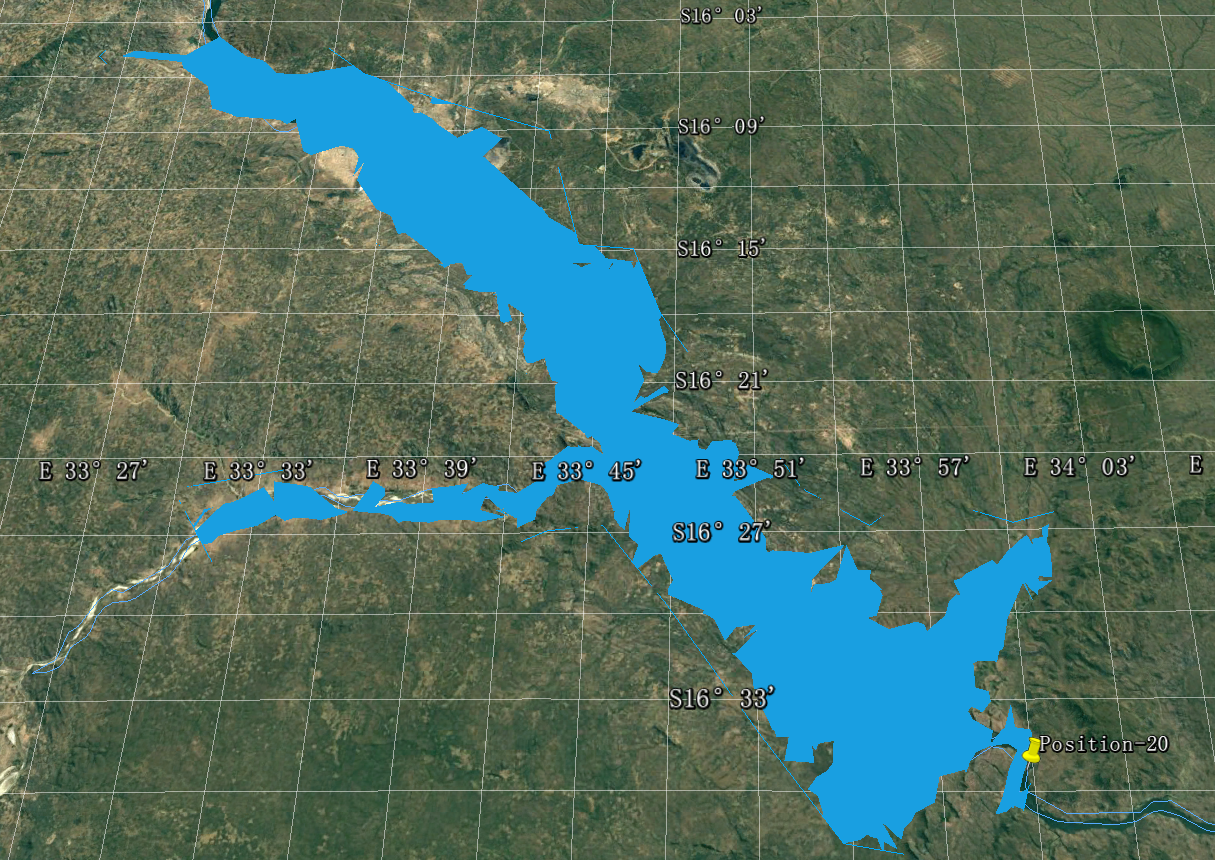
\includegraphics[width=8cm]{./figures/reservoir.png}
\caption{Effect diagram rendered by Google Earth} \label{fig:Fig1}
\end{figure}
\begin{figure}[htbp]
\centering %居中
\subfigure[Data of candidate locations]{ %第一张子图
\begin{minipage}{7cm}
\centering %子图居中
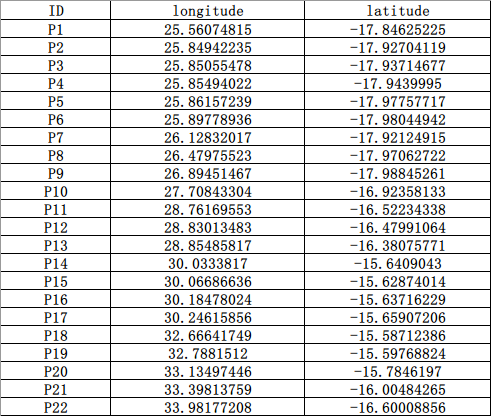
\includegraphics[scale=0.40]{figures/table_position.png} %以pic.jpg的0.5倍大小输出
\end{minipage}
}
\subfigure[Location of candidate points]{ %第二张子图
\begin{minipage}{7cm}
\centering %子图居中
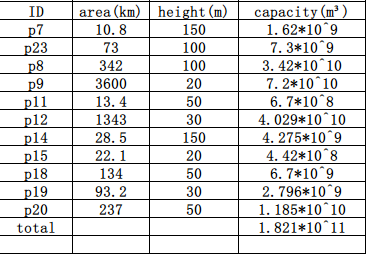
\includegraphics[scale=0.45]{figures/table_capacity.png} %以pic.jpg的0.5倍大小输出
\end{minipage}
}
\caption{Basic information on candidate points} % %大图名称
\label{fig:1.3.1} %图片引用标记
\end{figure}

\section{Model B : The Best Arrangement}
\subsection{Description}
\indent For a given dam system, a series of dam site selections and corresponding reservoir capacities, installed capacity, local precipitation limits, and so on, can already be determined. However, there are still many analyzes that can be carried out, among which the most interesting is the modulating of water resources between dams. The modulating scheme can protect the water resources and the benefits derived therefrom as much as possible on the basis of ensuring safety and responding to emergencies. It can be expected that the modulating scheme will be different in different situations (different periods in the water cycle, different water capacity of reservoirs, etc.). In order to cope with the different situations reasonably, a model of generating water resources modulating scheme is needed.\\

\subsection{Symbols}

\begin{table}[h]
\centering
  \begin{tabular}{cc}
  \hline
  Symbols & Meanings \\
  \hline
  $V$ & Water Resources Volume \\
  $V_{D}$ & The volume of water lost to the dam system as a result of flood discharge \\
  $V_{D,i}$ & The volume of water discharged from the reservoir $i$ during the unit time period.\\
  $\triangle V_{i}$ & Variation of Water Quantity per Unit Time in Reservoir $i$\\
  $V_{n, i}$ & The natural water increase in reservoir $i$ per unit time \\
  $V_{e, i}$ & The amount of water used per unit time for power generation of reservoir $i$\\
  $V_{u, i}$ & The amount of water in reservoir $i$ used for other purposes per unit of time \\
  $n$ & The number of dams in the Dam System, so the system also has $n$ reservoirs \\
  \hline
  \end{tabular}
\caption{Symbol Table of Model B}
\end{table}

\subsection{Assumptions}
\begin{enumerate}
  \item The use of water resources is divided into varieties, such as hydropower, agricultural irrigation, etc. In order to simplify the assessment of water resources value, we assume that the value of water resources is proportional to the volume of water resources $V$. 
  \item The amount of water lost to a dam system due to flood discharge can not be reused.
  \item The power generation water is transferred into the downstream reservoir, but the water for other uses is not directly transferred into the dam system.
\end{enumerate}

\subsection{Model Building}
\indent According to our first two assumptions, the value of water lost per unit time of a dam system is proportional to the amount of water lost due to flood discharge. And water is lost from the entire dam system only if it is drained as flood discharge from the last dam of the dam system, so we get
\begin{equation}
V_{D} = V_{D,n}
\end{equation}
\indent In order to maximize the benefits of the dam system, it is necessary to make the $ V_ {D, i} $ as small as possible, and the restrictive factors in different situations must be taken into account when proposing the modulating scheme. Therefore, we consider the use of optimization model to obtain water resources modulating scheme under certain case. \\
\indent According to our discussion above, the objective function of optimization is very simple, i.e.
\begin{equation}
\min V_{D} = V_{D, n}
\end{equation}
\indent In the following, we will focus on finding constraints. First, the amount of water in the reservoir after the unit time is equal to the sum of original amount of water, natural increment of the reservoir and drainage of upstream reservoirs (including power generation and flood discharge) then subtract the sum of water for other purposes, power generation and flood discharge, i.e.
\begin{equation} V_{i}^{'} =
\left\{
\begin{array}{cc}
 V_{i} + V_{n, i} + V_{D, i - 1} + V_{e, i - 1} - V_{u, i} - V_{e, i} - V_{D, i} & i > 1 \\
V_{i} + V_{n, i} - V_{u, i} - V_{e, i} - V_{D, i} & i = 1 \\
\end{array}
\right.
\end{equation}
where $ V_ {i} ^ {'} $ is the amount of water in reservoir $ i $ at the end of the period. 
$\triangle V = V ^ {'} - V $, then there have:
\begin{equation}
V_{n, i} =
\left\{
\begin{array}{cc}
\triangle V_{i} - V_{D, i - 1} - V_{e, i - 1} + V_{u, i} + V_{e, i} + V_{D, i} & i > 1 \\
\triangle V_{i} + V_{u, i} + V_{e, i} + V_{D, i}& i = 1 \\
\end{array}
\right.
\end{equation}
This is the equality constraint between variables

We consider more constraints on the variables
The Flood discharge capacity of the dam is clearly greater than or equal to zero and has an upper limit, ie
\begin{equation}
0 \leq V_{D, i} \leq V_{D, i}^{max}
\end{equation}
$ V_{D, i} ^ {max} $ is the maximum flood discharge capacity of dam $i$

Dam electricity generation capacity is limited, accordingly, the amount of water used for electricity generation is also limited. In addition, the amount of water used for electricity generation can not be negative, thus we get
\begin{equation}
0 \leq V_{e, i} \leq V_{e, i}^{\max}
\end{equation}

Similarly, for $ V_ {u, i} $ we have:
\begin{equation}
V_{u, i}^{\min} \leq V_{u, i} \leq V_{u, i}^{\max}
\end{equation}

\indent The lower limit of $ V_ {u, i} $ is not $ 0 $, considering that the rigid demand for agricultural water use around the reservoir.\\
\indent The constraint on $ \triangle V_ {i} $ should depend on the reservoir's existing water volume, future plans for reservoir volumes, and natural replenishment of future reservoirs. But intuitively, the water level of the reservoir should not be violent fluctuations; and our model should allow professionals to give limits of the reservoir water level fluctuations where used in specific case in the relevant areas, so we express the constraints of $ \triangle V_ {i} $ as:
\begin{equation}
\alpha_{i} \leq \frac{\triangle V_{i}}{V_{i}^{\max}} \leq \beta_{i}
\end{equation}
where $ V_ {i} ^ {\ max} $ is the maximum volume of the reservoir.

\indent Although some dams in the system can stop generating electricity at a certain time due to the regulation of the power grid, considering the need to meet the electricity needs of the local and other areas, the total generation of the dam system should have a lower limit of more than $ 0 $, thus we get:
\begin{equation}
\sum_{i = 1}^{n} V_{e, i} \geq E_{min}
\end{equation}
$ E_ {min} $ is the amount of water required to produce the minimum electricity demand.

\subsection{Macro Plan of Water Resources modulating}
Based on the characteristics of the dam system obtained in Model A and the experience of dam management, we have proposed the following macro scenario for water resources modulating. The scenario can guide the staff of the River Authority to choose different values of $\alpha_{i}$ and $\beta_{i}$ under different circumstances. Then, the optimal scheduling scheme of water resources is obtained by solving the above model. It is observed that in the dam system we get, the reservoirs with large volume have smaller drops than that with small volume and the reservoirs with small volume usually have larger drops. That is, the smaller reservoirs have more potential in energy generation, so we need them to run in a water level as high as possible. However, the big reservoir should drain some water ahead of the rainy season to make sure it safety when the flood is coming. Based on the factors above, we think the macro plan should have several principles as follow:
\begin{itemize}
  \item In the dry season, the reservoir in upstream should reduce the power generation to ensure other water need.
  \item In the rainy season, the reservoir in the midstream should catch the water from upstream and reduce the flood discharge pressure of downstream. Meanwhile, the the reservoir in upstream and downstream should keep in safety water level.
  \item To the small dams in midstream, do the same activity as small reservoirs in downstream.
\end{itemize}
Change the principles above into the choose of $\alpha_{i}$ and $\beta_{i}$:
\begin{itemize}
  \item To the small reservoir along the river, we should choose bigger $\alpha_{i}$ in the rainy season and smaller $\beta_{i}$ in rainy season.
  \item To the big reservoir in the midstream, choose smaller $\beta_{i}$ in the dry season.
\end{itemize}
The choose above makes the water level of small dams remains high in the dry season and make it possible to storage the water that cannot be used in the rainy season, which improves the utilization of water resources. Meanwhile, the schedule above performs well in emergency.
\subsection{Result}
Choosing values for $ \alpha_ {i} $ and $ \beta_ {i} $ in a variety of situations is a complex task. We believe that their value should be estimated by professionals in practice. However, according to the monthly flow data of Zambezi River, the average monthly precipitation, monthly evaporation and other data, we still can get the better values of $ \alpha, \beta $ in different situations by simulation of the model. 

To simulate the model, we need to determine the value of the model parameters, we estimate the installed capacity of the reservoir by the following equation $V_{e, i}$:
\begin{equation}
V_{e, i} = \frac{V_{total}t}{\eta \rho gH_{i}}
\end{equation}
the parameter t represents the length of time.

For the most upstream reservoirs, the main factors influencing the natural increment of the reservoirs are the upstream runoff, the regional precipitation and the evaporation loss. For the other reservoirs, the main factors influencing their natural increment are the area precipitation and evaporation loss, which is:

\begin{equation}
V_{n,i} = \left\{
\begin{array}{cc}
V_{flow,i} - V_{evap,i} + V_{rain,i} & i = 1 \\
-V_{evap,i} + V_{rain,i} & i > 1 \\
\end{array}
\right.
\end{equation}

According to the experience, we estimate the value of $E_{m}$ as:
\begin{equation}
E_{m} = 30\%\sum V_{n, i}
\end{equation}

Based on the model B described above, we have programmed according to the above-mentioned parameters selection principles and the dam situation. The climatic data of normal years, drought years and flood years were obtained by referring to the data, and the parameters such as precipitation, flux, evaporation, water consumption and so on. According to the iterative adjustment of the value of $ \alpha, \beta $, three optimal selection schemes are obtained to reflect the scheduling strategy of the dam system under different conditions.

In order to simplify the model, we divided the reservoir scheduling behavior to maintain the water level, lower water levels, improve the water level. Through the simulation of the model, we get the following $ (\alpha, \beta) $ value:

\begin{table}[!hbp]
\centering
\begin{tabular}{|c|c|c|c|}
\hline
  & Normal & Drought & Flood \\
\hline
maintain the water level& (-0.05, 0.05) & (-0.03, 0.06) & (-0.07, 0.03) \\
\hline
lower the water level& (-0.02, 0.1) & (0.01, 0.1) & (-0.05, 0.1)  \\
\hline
improve the water level& (-0.1, 0.02) & (-0.08, 0.04) & (-0.1, 0.01) \\
\hline
\end{tabular}
\end{table}


\section{Strengths and weaknesses}
\subsection{Model A: Search for possible locations to build dams}
Model A has the following weaknesses.
\begin{itemize}
\item When building the benchmark function, some factors can not be quantified which will bring some errors.
\item In the rough selection of the candidate areas, some of the valuable points may be ignored, resulting in the non-optimal solution.
\end{itemize}
Despite of the weakness, it has more strengths.
\begin{itemize}
  \item The factors considered in this model are rather comprehensive. The benchmark function can be a good reflection of the impact of various factors.
  \item Using the analytic hierarchy process(AHP) to find the final solution, the result is accurate.
  \item The established benchmark function has a good guiding role for address selection.
  \item The specific dam construction plan is obtained, and the requirement of water storage capacity can be satisfied. Meanwhile, the multi-dam system have great advantage in adjusting the flow of Zambezi River basin.
\end{itemize}

\subsection{Model B: The Best Arrangement}
In Model B, we consider that the objective function of the optimization model is simplified to a relatively large extent and the given reference parameters may not be optimal for a particular case, which are weaknesses. However we have more strengths as below:
\begin{itemize}
  \item The model can be adjusted by a professional.
  \item The model gives the global optimal solution under certain constraints.
  \item The reference parameters for controlling the reservoir water volume in usual, drought and flood years are given.
\end{itemize}

\section{Conclusion}
\indent \indent In model A, we firstly analyzed the elevation along Zambezi River. Combined with other geography factors, we found some candidate areas to build new small dams. According to our research result, the new dams should be concentrated in the middle and lower reaches of the Zambezi River, which is the basis of our next step. After that, we established a benchmark function to evaluate the candidate locations. This function is built by using AHP, which combine various important factors such as terrain conditions, construction cost, income and safety. We evaluated a series of specific locations by using this function and selected the candidate points with higher scores to build our new dam system.\\
\indent Having chosen the specific locations, we further discussed the modulating strategy of our multi-dam system in face of complex conditions. Since the water level of Zambezi River changes intensely in a year, we anticipate that it is very difficult to obtain a unified scheduling scheme directly. So, we consider whether we can get a model to generate a specific scheduling strategy. This model should generate the corresponding optimal scheduling scheme according to the specific situation. We first establish a linear model with a global optimal solution under certain constraints. Moreover, we considered the action of people and take it as a parameter. After that, we use the historical data to simulate and get the value of parameters in normal year, in the dry season and rainy season.

\begin{thebibliography}{99}
\bibitem{1} IRMSA , Impact of the failure of the Kariba Dam, June 2015.
\bibitem{2} Welcomme, R.L., 1985. River fisheries. FAO Fish. Tech. Pap. No. 262, Rome.
\bibitem{3} Zhou Houqing. A mathematic model of the spread of ebola. Journal of Shaoyang
University(Natrual Science Edition), (1672-7010(2014)04-0001-05), 12 2014.
\bibitem{4} WIKIPEDIA Zambezi River, Lake Kariba, Dam Kariba
\bibitem{5} The estimation of dam building cost, Ni Ruzhou, Hydro Review, 2007
\bibitem{6} Decision making with the analytic hierarchy process, Thomas L. Saaty, Services Sciences, 2008
\bibitem{7} Dam site selection using an integrated method of AHP and GIS for decision making support in Bortala, Northwest China, XinyiDai, Lund University GEM thesis series, 2016
\bibitem{8} The Zambezi River, Andy E. Moore 1 , Fenton P.D. (Woody) Cotterill, 2007
\end{thebibliography}

\clearpage
\section{Brief Assessment of the options}
\indent \indent The solution to the Kariba Dam problem can simply be divided into three options: repairing it, rebuilding it or removing it then replacing it with other dams. To the third method, ZRA suggests to build $10\sim20$ small dams to replace the huge Kariba Dam.\\
\indent Evaluating the options from the perspective of cost and benefit is a complex task, since it can be influence by a number of factors. Only considering the cost of building dams, although it can be estimated accurately by using the cost formula below \\
\[C_{p} = K\left(\frac{V}{\left(\frac{H}{0.3}\right)^{0.3}}\right)^{0.82}\]
where $C_{p}$ is the cost of building the hydropower station, $V$ is the installed capacity, $H$ is the design head, $K$ is the proportional coefficient. However, the ecological costs of dam construction need to be considered more cautiously because damage to the ecological environment may be irreversible.\\
\indent Option 1. Repairing the existing Kariba Dam. This is the option with the lowest cost of construction. Meanwhile, it won't change the submerged area, so there is no extra ecological cost. From the aspect of revenue, the reconstruction and expansion of Kariba Dam hydropower station can be carried out at the same time, which can effectively increase the total installed capacity of hydropower station, and thus improve the income of hydropower station. In fact, the expansion of the Kariba Dam hydropower station is underway. Since the reconstruction will not affect the Kariba Lake, the benefits from the use of water from the lake won't be reduced. The analysis above is based on the assumption that the climate will not change drastically in the future and no rare disasters which is outside the historical statistics will occur.\\
\indent Option 2. Rebuilding the existing Kariba Dam. Because rebuilding the Kariba Dam need to remove the existing the dam and rebuild it at the origin site, it is an option with high risk and cost. What's more, the reconstruction of the dam will inevitably lead to the result that the hydropower station can't generate electricity in quite a long period, so this part of loss should also be included in the cost of reconstruction. However, rebuilding dams do have benefits. It helps to expand the installed capacity of hydropower station (benefit from re-designing the internal structure and using more advanced equipment). The new designed Dam would have better flood protection capacity, which allows river management to handle emergency with more flexibility. Stronger water storage capacity means we can raise the water level of Kariba Lake. It will increase the energy generation as well as bring the risk of ecologic damage which needs to be treated with caution.\\
\indent Option 3. Removing the Kariba Dam and replacing it with a series of $10\sim20$ smaller dams along the Zambezi River. This is quite an ambitious plan. Even if the sum of installed capacity of all these small dams is the same as that of Kariba Dam, the total construction cost is still expected to be higher than rebuilding Kariba Dam according to the cost formula above. With the same problem as option 2, removing Kariba Dam will definitely lead to the loss of energy generation, furthermore even the construction of a smaller dam in the original position of Kariba Dam may result in loss of water storage capacity, as the water level in Kariba Lake will decrease. Fortunately, these losses can be minimized through rational planning. Specifically, we can give priority to the construction of small dams, and then gradually replace the Kariba Dam with their power generation capacity. New dams built in the down stream would store the water from Kariba Dam when it is removed, which can reduce the loss of water resources. Different from the previous two options, economic compensation of the new reservoirs' reserved area also needs to be include in the cost.(Here we can make an estimate by calculating the unit area GDP of the catchment)From the ecological point of view, the third option is also accompanied by greater risk. It will not only flood new areas, but also affect the ecology of Lake Kariba (the water level drops and the lake is divided into several parts). In terms of revenue, the scheduling of water resources between dams will reduce the loss of water resources caused by flooding discharge, which will actually help to increase the power generation capacity of hydropower stations. Moreover, the rational allocation of flood storage between dams will increase the safety of the dam system, the reduced reservoir area will reduce the evaporation loss of water and, in the face of emergencies, river management can also adopt a more flexible approach. Because of the high cost of the third option, a long-term analysis is of great significance. In the future, the flow of Zambezi River may reduce by $40\%\sim50\%$ due to the climate change. Although the climate predictions nowadays are with a large degree of uncertainty, but we should never be blindly optimistic about the benefits of the new dam system.\\

% \clearpage
% \begin{appendices}

% \section{First appendix}

% \lipsum[13]

% Here are simulation programs we used in our model as follow.\\

% \textbf{\textcolor[rgb]{0.98,0.00,0.00}{Input matlab source:}}
% \lstinputlisting[language=Matlab]{./code/mcmthesis-matlab1.m}

% \section{Second appendix}

% some more text \textcolor[rgb]{0.98,0.00,0.00}{\textbf{Input C++ source:}}
% \lstinputlisting[language=C++]{./code/mcmthesis-sudoku.cpp}

% \end{appendices}

\end{document}